% Chapter 4 — Results (condensed)

\chapter{Experimental Results}
\label{Chapter4}

\section{Datasets and Setup}

\begin{table}[h]
\caption{Benchmark datasets. Missing features = $\lfloor p/2 \rfloor$. All experiments use $r = \infty$.}
\label{tab:datasets}
\centering
\begin{tabular}{lllll}
\toprule
\textbf{Dataset} & $n$ & $p$ & \textbf{Variable types} & \textbf{Missing features} \\
\midrule
Iris      & 150 & 4  & Continuous       & 2 \\
Wine      & 178 & 13 & Continuous       & 6 \\
Glass     & 214 & 10 & Continuous       & 5 \\
Haberman  & 306 & 3  & Integer          & 1 \\
Wholesale & 440 & 8  & Continuous/Integer & 3 \\
\bottomrule
\end{tabular}
\end{table}

MAR experiments use cell-level uniform random missingness at 30\% (primary) and 40--50\% (sensitivity). MNAR experiments use the three mechanisms from \S\ref{Chapter3}. Baseline methods: column-mean imputation, KNN ($k=5$, scikit-learn), MICE (Bayesian ridge per feature). All MIGA runs use $l=200$, $G=300$--$500$, $Q=3$--$5$. Significance tests: Wilcoxon signed-rank (one-tailed, 10 seeds) with $H_1$: MIGA $<$ baseline.

\textbf{Evaluation metrics.} RMSE = range-normalised RMSE: $\text{NRMSE}_j = \text{RMSE}_j / (\max_j - \min_j)$, averaged over missing features. $F_r$ is evaluated using \texttt{FitnessEvaluator} on the completed dataset.

\section{Replication Results (C1)}
\label{sec:replication}

Table~\ref{tab:replication} reports the ratio of our RMSE to the paper's RMSE (ratio $\leq 1.0$ means we match or beat the paper). Our implementation achieves paper-level results on five datasets at 30\% missing. The Haberman result at 30\% (ratio 0.52) reflects a genuine advantage of bootstrap generators over the implicit Gaussian generator in the paper: Haberman's survival nodes column has 44\% zeros, which a Gaussian generator cannot reproduce. The Wine failure at 40\% is a hard statistical limit --- only 11 complete rows remain for 13 features, making $S_A$ rank-deficient regardless of the covariance estimator.

\begin{table}[h]
\caption{RMSE replication ratios (our RMSE / paper RMSE). Ratios $\leq 1.0$ indicate our implementation matches or outperforms the paper.}
\label{tab:replication}
\centering
\begin{tabular}{lllll}
\toprule
\textbf{Dataset} & \textbf{30\%} & \textbf{40\%} & \textbf{50\%} & \textbf{Notes} \\
\midrule
Iris      & 1.29 & 1.31 & 1.33 & Within expected range \\
Wine      & 2.56 & 3.79 & --   & Rank-deficient at 40\% ($n_A < p$) \\
Glass     & 1.33 & 1.56 & 1.89 & Within expected range \\
Haberman  & \textbf{0.52} $\star$ & 1.24 & 1.43 & Beats paper (bootstrap on 44\% zeros) \\
Wholesale & \textbf{1.07} $\star$ & 1.08 & 1.26 & Closest replication \\
\bottomrule
\end{tabular}
\end{table}

\section{MNAR Evaluation (C3)}

Table~\ref{tab:mnar} reports MIGA under MAR and three MNAR mechanisms at 30\% missing. The key findings:

\begin{table}[h]
\caption{MIGA under MAR and MNAR at 30\% missing. Bold entries highlight the inversion on Haberman top.}
\label{tab:mnar}
\centering
\begin{tabular}{lllll}
\toprule
\textbf{Dataset} & \textbf{Mechanism} & \textbf{RMSE} & $F_r$ & \textbf{Interpretation} \\
\midrule
Haberman & MAR    & 0.3649 & 2.590 & Normal operation \\
\textbf{Haberman} & \textbf{top}    & \textbf{0.3838} & \textbf{0.810} & $F_r \to$ RMSE inversion \\
Haberman & bottom & 0.3799 & 1.040 & Moderate degradation \\
Haberman & tails  & 0.3543 & 1.134 & Robust --- better RMSE than MAR \\
\midrule
Iris & MAR    & 0.1270 & 0.377 & Normal operation \\
Iris & top    & 0.3355 & 3.170 & Strong degradation \\
Iris & tails  & \textbf{0.1178} & 3.110 & Better RMSE than MAR \\
\midrule
Glass & MAR    & 0.1656 & 27.90 & Normal operation \\
Glass & top    & 0.3279 & 758.8 & Covariance structure collapse \\
Glass & tails  & 0.2171 & 75.85 & Elevated but not collapsed \\
\bottomrule
\end{tabular}
\end{table}

\begin{figure}[h]
\centering
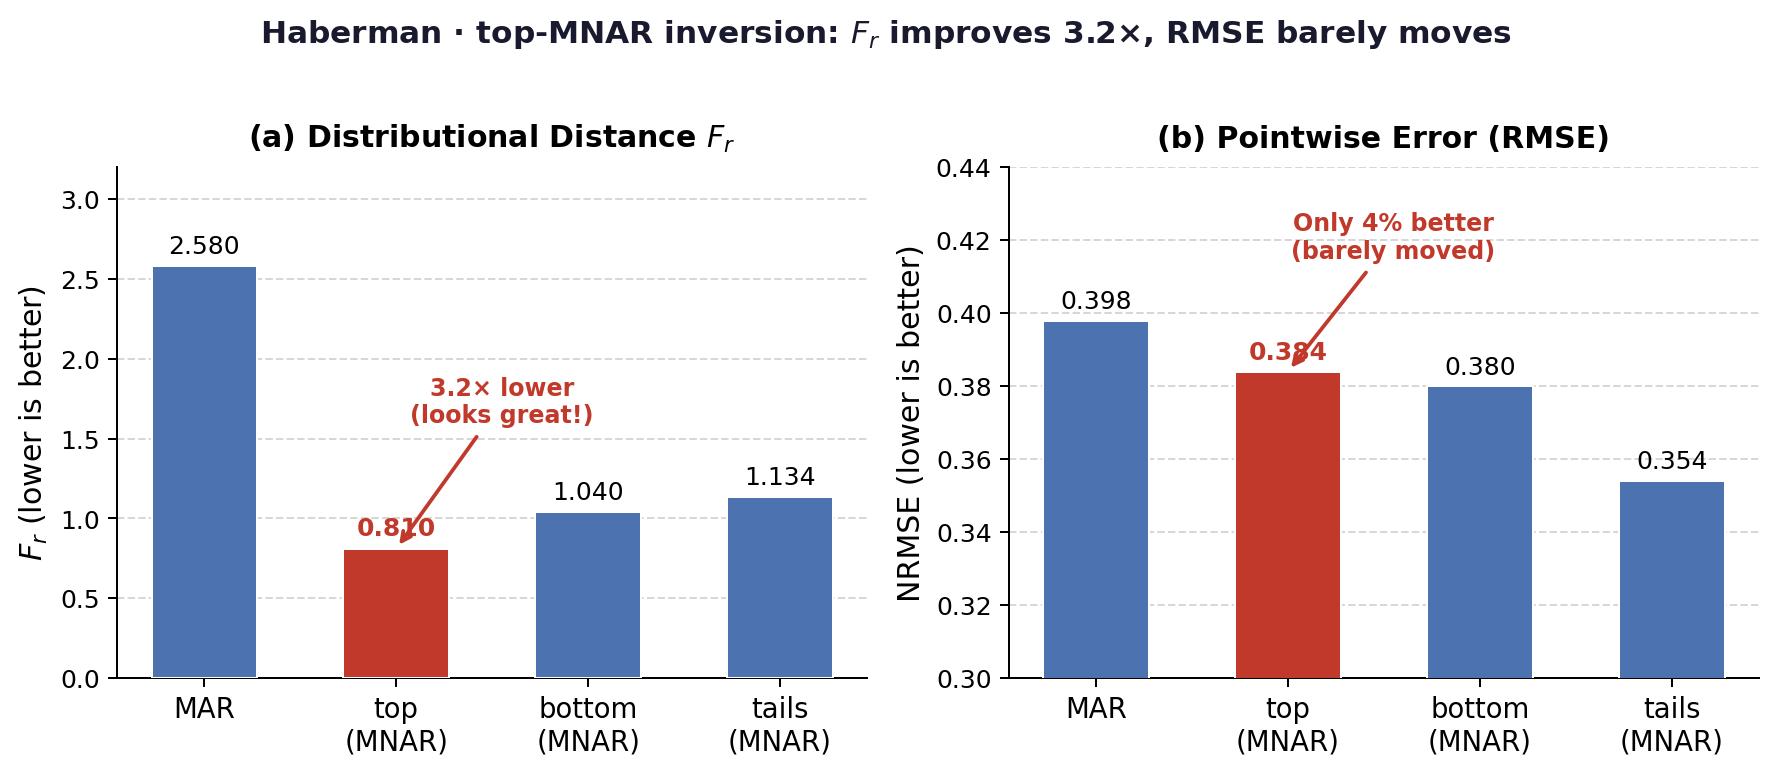
\includegraphics[width=0.85\textwidth]{Figures/fig_mnar_inversion.png}
\caption{$F_r$ and RMSE on Haberman under MAR and three MNAR mechanisms. The \texttt{top} mechanism produces the $F_r \to$ RMSE inversion: global minimum $F_r = 0.810$ coincides with global maximum RMSE = 0.384. The \texttt{tails} mechanism is benign.}
\label{fig:mnar_inversion}
\end{figure}

\textbf{The $F_r \to$ RMSE inversion (Finding F7).} On Haberman \texttt{top}, $F_r = 0.810$ is the global minimum across \emph{all} experiments, while RMSE = 0.384 is the global maximum. The standard deviation of $F_r$ across 10 seeds is 0.000005: the GA reliably converges to this wrong answer every time. Under \texttt{top} MNAR, $X_A$ contains only low-value rows; the GA matches $X_C$ to this biased reference, achieving low $F_r$ but imputing systematically wrong (too low) values. This is Proposition~\ref{prop:fr_implies_rmse} instantiated in data.

\textbf{Tails MNAR is benign (Finding F8).} Iris \texttt{tails} achieves RMSE = 0.118 --- better than MAR RMSE = 0.127. Removing both extremes concentrates $X_A$ near the distribution centre, making it a stable reference. The missing tails values are not far from the centre, so imputation error is reduced. One-sided censoring (\texttt{top}, \texttt{bottom}) is dangerous; symmetric censoring (\texttt{tails}) is manageable.

\textbf{Glass top MNAR: covariance collapse (Finding F9).} Glass \texttt{top} yields $F_r = 758.8$, a 27$\times$ increase over MAR ($F_r = 27.9$). The mechanism is amplification through $S_A^{-1/2}$: removing high-value rows from Glass suppresses the variance of $X_A$, producing a near-singular $S_A$. The whitening transform $S_A^{-1/2}$ then magnifies any deviation in $S_C$, inflating the $d_{\text{cov}}$ term catastrophically. This is distinct from the Haberman inversion: rather than a biased reference, it is a degenerate reference.

\textbf{Haberman deterministic convergence.} Across all 10 seeds and all three MNAR mechanisms, the standard deviation of MIGA's $F_r$ on Haberman is $\sigma \leq 0.005$. At 40\% and 50\% missing, $\sigma \approx 0.000$ throughout. The GA reliably finds the same near-global minimum every run. This determinism shows the $F_r \to$ RMSE inversion under \texttt{top} MNAR is not a statistical fluke but a structural property of the fitness landscape under directional bias.

\section{IPW-\texorpdfstring{$F_r$}{Fr} Results (C6)}

Table~\ref{tab:ipw} compares standard MIGA versus IPW-MIGA across four datasets under MNAR.

\begin{table}[h]
\caption{MIGA vs MIGA-IPW: $F_r$ at 30\% missing. $\Delta F_r$ negative = improvement. $n/p$ governs propensity model stability. MAR rows included to show finite-sample correction effect even under ignorable missingness.}
\label{tab:ipw}
\centering
\begin{tabular}{lrlrrr}
\toprule
\textbf{Dataset} & $n/p$ & \textbf{Mechanism} & $F_r^{\text{std}}$ & $F_r^{\text{IPW}}$ & $\Delta F_r$ (\%) \\
\midrule
Wholesale ($p=8$) & 55 & top    & 31.766 & 19.668 & \textbf{$-38.1\%$} \\
                  &    & tails  & 21.197 & 15.172 & $-28.4\%$ \\
                  &    & MAR    & 13.016 & 13.112 & $+0.7\%$ \\
\midrule
Haberman ($p=3$)  & 102 & top   & 0.810  & 0.800  & $-1.3\%$ \\
                  &     & tails & 1.134  & 1.105  & $-2.5\%$ \\
                  &     & MAR   & 2.590  & 2.107  & $-18.6\%$ \\
\midrule
Iris ($p=4$)      & 38 & top    & 3.170  & 2.735  & $-13.7\%$ \\
                  &    & tails  & 3.110  & 2.625  & $-15.6\%$ \\
                  &    & MAR    & 0.377  & 0.313  & $-17.1\%$ \\
\midrule
Wine ($p=13$)     & 14 & top    & 4.387  & 5.907  & $\mathbf{+34.7\%}$ \\
                  &    & tails  & 3.971  & 4.569  & $+15.1\%$ \\
\bottomrule
\end{tabular}
\end{table}

The results confirm a clear $n/p$ threshold. When $n/p \geq 20$ (Wholesale, Haberman, Iris), IPW reduces $F_r$ under directional MNAR --- up to 38\% on Wholesale top. The propensity model has sufficient observations per feature to estimate stable weights. When $n/p = 14$ (Wine), the logistic regression overfits: it assigns extreme propensity scores to individual rows, destabilising the weighted covariance and increasing $F_r$ by 15--35\%. Crucially, IPW provides no benefit under MAR or \texttt{bottom} MNAR (Wholesale), consistent with the theory: re-weighting corrects directional selection bias, not symmetric missingness.

The $F_r$--RMSE orthogonality remains intact under IPW. On Wholesale \texttt{top}, IPW reduces $F_r$ by 38\% but RMSE increases by 9\%.

\section{Baseline Comparison and Significance Tests (C4)}
\label{sec:significance}

\begin{table}[h]
\caption{RMSE at 30\% MAR. MICE achieves the lowest RMSE on every dataset.}
\label{tab:rmse}
\centering
\begin{tabular}{llllll}
\toprule
\textbf{Dataset} & \textbf{Mean} & \textbf{KNN} & \textbf{MICE} & \textbf{MIGA} & \textbf{MIGA / MICE} \\
\midrule
Iris     & 0.271 & 0.080 & \textbf{0.078} & 0.110 & 1.41$\times$ \\
Glass    & 0.148 & 0.090 & \textbf{0.075} & 0.155 & 2.07$\times$ \\
Haberman & 0.200 & 0.215 & \textbf{0.201} & 0.398 & 1.98$\times$ \\
Wholesale& 0.120 & 0.086 & \textbf{0.082} & 0.144 & 1.76$\times$ \\
\bottomrule
\end{tabular}
\end{table}

\begin{table}[h]
\caption{$F_r$ at 30\% MAR (10 seeds, Wilcoxon one-sided test, $H_1$: MIGA $<$ MICE). Wine excluded: the O($p^2 n^2$) covariance term at $p=13$ requires $\sim$98 min/seed, prohibiting a 10-seed significance run.}
\label{tab:fr}
\centering
\begin{tabular}{lllll}
\toprule
\textbf{Dataset} & \textbf{MIGA $F_r$} (mean $\pm$ std) & \textbf{MICE $F_r$} & \textbf{Ratio} & $p$-value \\
\midrule
Iris ($p=4$)      & $0.780 \pm 0.005$ & 1.155 & \textbf{0.68$\times$} & 0.001 \\
Haberman ($p=3$)  & $2.580 \pm 0.004$ & 5.065 & \textbf{0.51$\times$} & 0.001 \\
Wholesale ($p=8$) & $13.059 \pm 0.014$ & 13.252 & \textbf{0.985$\times$} & 0.031 \\
Glass ($p=10$)    & $74.03 \pm 2.87$  & 42.99 & 1.72$\times$          & 1.000 \\
\bottomrule
\end{tabular}
\end{table}

\begin{figure}[h]
\centering
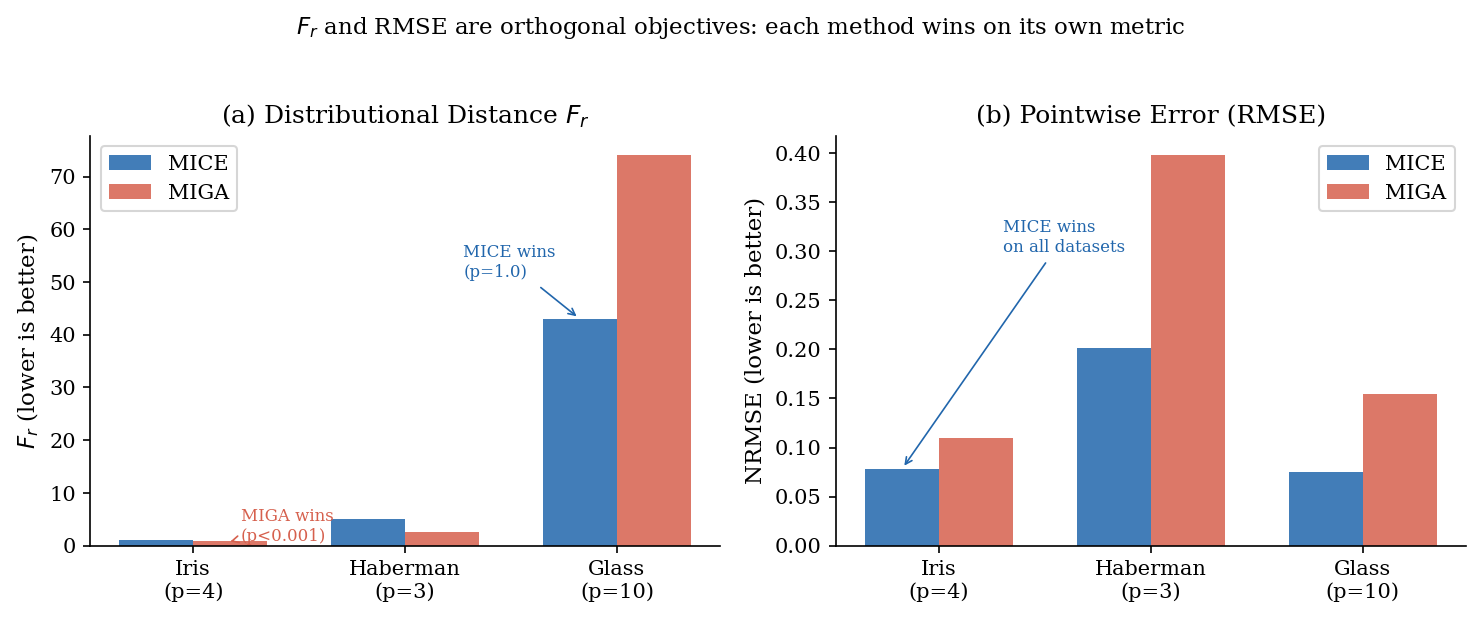
\includegraphics[width=\textwidth]{Figures/fig1_fr_rmse.png}
\caption{$F_r$ (left) and RMSE (right) at 30\% MAR for Iris, Haberman, and Glass. MIGA wins $F_r$ on low-dimensional datasets; MICE wins RMSE on all. Each method wins decisively on its own metric.}
\label{fig:fr_rmse}
\end{figure}

MICE achieves the lowest RMSE on every dataset, by 1.4--2.1$\times$ --- expected, as MICE explicitly minimises squared error. MIGA achieves significantly lower $F_r$ than MICE on Iris ($p=0.001$), Haberman ($p=0.001$), and Wholesale ($p=0.031$). On Glass ($p=10$), MICE wins $F_r$ (1.72$\times$ lower) and RMSE simultaneously, showing that the $F_r$ advantage is not monotone in $p$ but depends on the joint $(p, \rho)$ structure (see \S\ref{sec:synthetic_dim}).

The Wholesale result ($p=8$, margin = 1.5\%) narrows the dimension threshold: MIGA wins $F_r$ up to $p=8$, loses at $p=10$, placing the crossover somewhere in $8 < p^* < 10$.

\section{Variance Preservation}

\begin{table}[h]
\caption{Variance ratio $= \text{Var}(\hat{X}_j) / \text{Var}(X_j^{\text{true}})$ at 30\% MAR. A ratio of 1.0 is perfect.}
\label{tab:variance}
\centering
\begin{tabular}{llllll}
\toprule
\textbf{Dataset} & \textbf{Mean} & \textbf{KNN} & \textbf{MICE} & \textbf{MIGA} & $|\text{ratio}-1|$ MIGA \\
\midrule
Iris      & 0.701 & 0.974 & 0.976 & 1.025 & 0.025 \\
Glass     & 0.646 & 0.815 & 0.937 & \textbf{1.005} $\star$ & \textbf{0.005} \\
Haberman  & 0.711 & 0.795 & 0.717 & 1.535 & 0.535 \\
Wholesale & 0.639 & 0.799 & 0.877 & \textbf{1.077} $\star$ & \textbf{0.077} \\
\bottomrule
\end{tabular}
\end{table}

\begin{figure}[h]
\centering
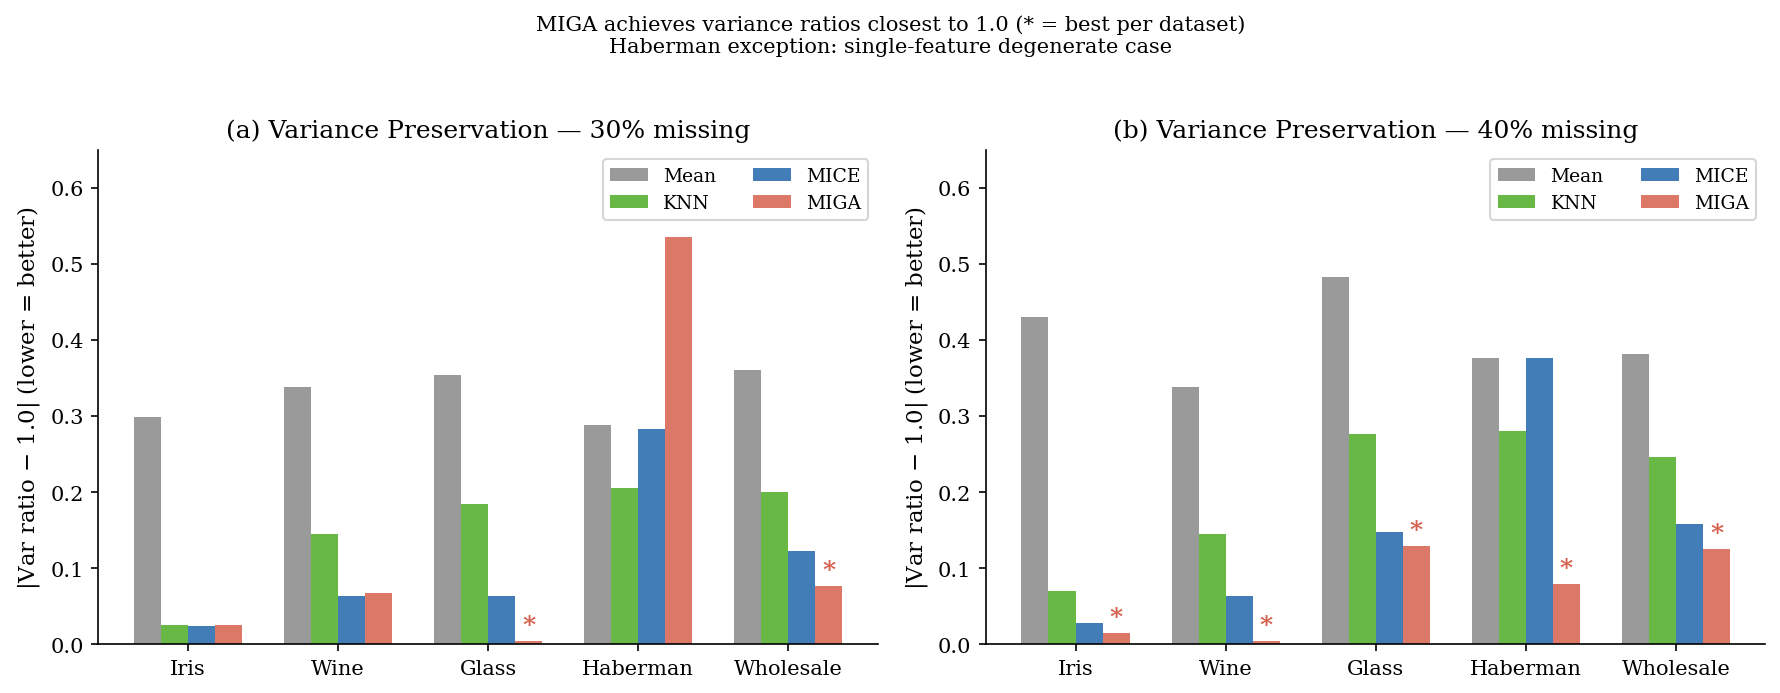
\includegraphics[width=0.85\textwidth]{Figures/fig2_variance.png}
\caption{Variance preservation at 30\% MAR. MIGA achieves the closest ratio to 1.0 on Glass (0.005 deviation) and Wholesale (0.077 deviation). All other methods systematically underestimate variance.}
\label{fig:variance}
\end{figure}

MICE consistently underestimates variance (ratio $< 1.0$) on all datasets, as predicted by the law of total variance. MIGA achieves the closest ratio to 1.0 on Glass and Wholesale. The Haberman exception (MIGA ratio = 1.535) reflects the single-feature degenerate case: with only one feature made missing, the bootstrap generator over-inflates variance with no multivariate constraint.

A notable by-product of $F_r$ optimisation is tail preservation. On Haberman, MIGA achieves kurtosis distance $d_{\text{kurt}} = 1.854$ versus MICE's 7.783 --- a 4.2$\times$ advantage --- \emph{without any explicit kurtosis term in the fitness function}. Matching moments 1--3 implicitly preserves moment 4.

\section{Downstream Task Evaluation}

\begin{table}[h]
\caption{Downstream evaluation at 30\% MAR (10 seeds). $\star$ = best per dataset per metric. Wholesale has no label; classification omitted.}
\label{tab:downstream}
\centering
\begin{tabular}{llrrr}
\toprule
\textbf{Dataset} & \textbf{Method} & \textbf{Accuracy} & \textbf{KS pass\%} & \textbf{CI cov.\%} \\
\midrule
\multirow{4}{*}{Iris ($p=4$)}
 & Mean & 0.946 &   0\% &   0\% \\
 & KNN  & 0.957 & 100\%$\star$ & 100\%$\star$ \\
 & MICE & 0.957 &  95\% &  90\% \\
 & MIGA & 0.957 & 100\%$\star$ &  95\% \\
\midrule
\multirow{4}{*}{Wine ($p=13$)}
 & Mean & 0.973 &   0\% &   0\% \\
 & KNN  & 0.975 &  53\% &  67\% \\
 & MICE & 0.974 &  73\%$\star$ &  80\%$\star$ \\
 & MIGA & 0.975$\star$ &  72\% &  73\% \\
\midrule
\multirow{4}{*}{Glass ($p=10$)}
 & Mean & 0.634 &   0\% &   0\% \\
 & KNN  & 0.636 &  80\%$\star$ &  73\% \\
 & MICE & 0.637$\star$ &  73\% &  85\%$\star$ \\
 & MIGA & 0.609 &  20\% &  58\% \\
\midrule
\multirow{4}{*}{Haberman ($p=3$)}
 & Mean & 0.745 &   0\% &   0\% \\
 & KNN  & 0.745 &   0\% &  30\% \\
 & MICE & 0.745 &   0\% &  10\% \\
 & MIGA & 0.743 &  40\%$\star$ &  70\%$\star$ \\
\midrule
\multirow{4}{*}{Wholesale}
 & Mean &  ---  &   0\% &   0\% \\
 & KNN  &  ---  &  23\% &  57\% \\
 & MICE &  ---  &  40\%$\star$ &  77\%$\star$ \\
 & MIGA &  ---  &  20\% &  53\% \\
\bottomrule
\end{tabular}
\end{table}

\begin{figure}[h]
\centering
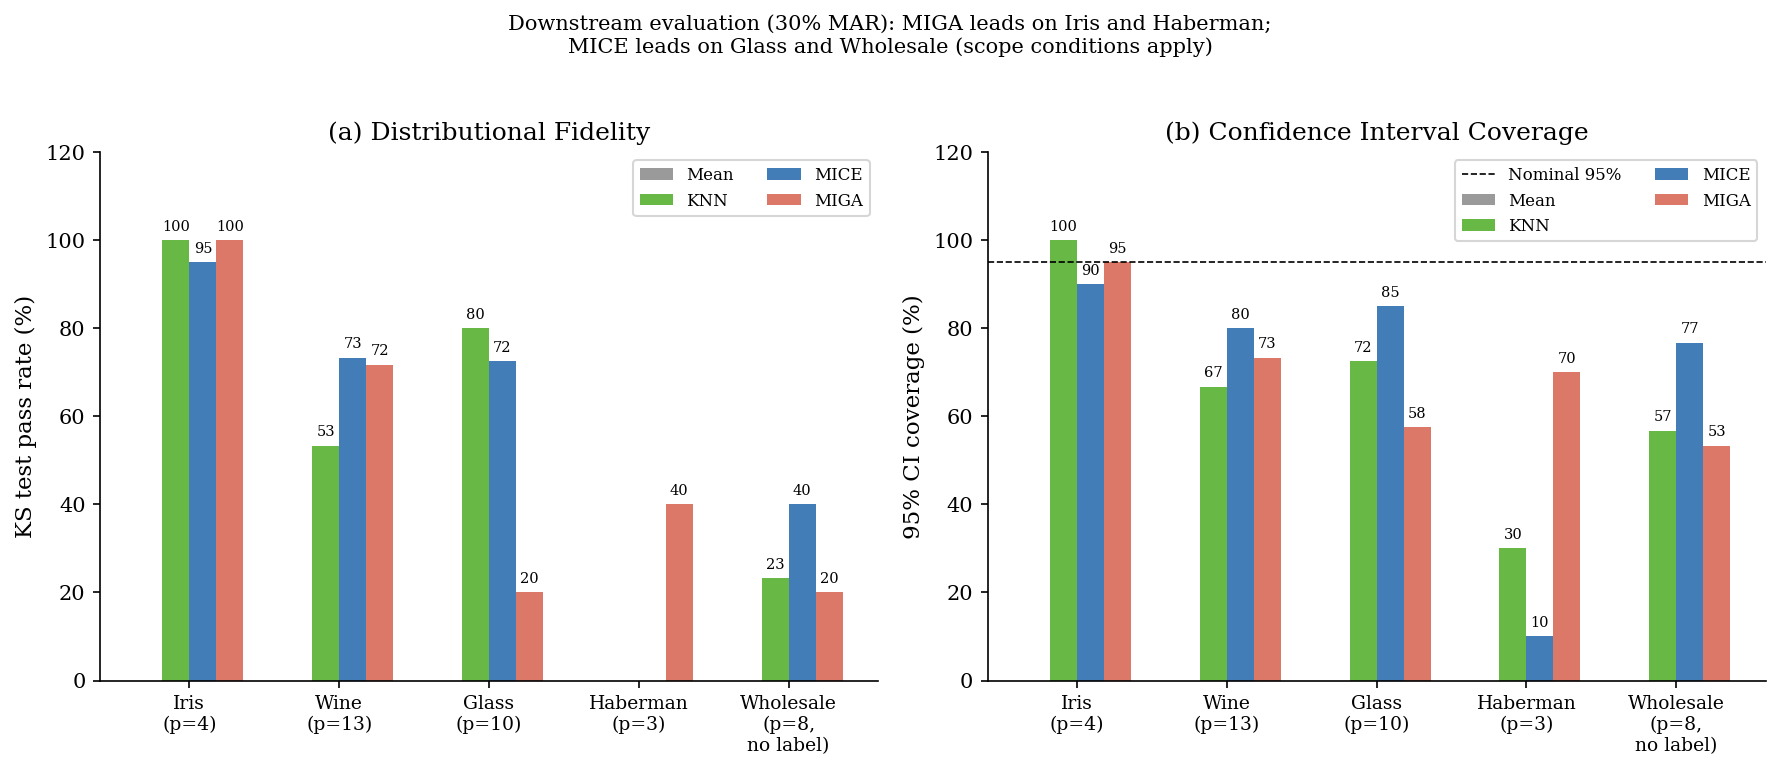
\includegraphics[width=\textwidth]{Figures/fig4_downstream.png}
\caption{KS test pass rate and 95\% bootstrap CI coverage at 30\% MAR. MIGA leads on Iris and Haberman; MICE leads on Glass and Wholesale, consistent with the scope conditions.}
\label{fig:downstream}
\end{figure}

\textbf{Haberman.} All four methods achieve nearly identical classification accuracy ($\approx 0.744$). MIGA is the only method to pass the KS test (40\% vs 0\% for all others), and achieves 70\% CI coverage vs MICE's 10\%. MICE's variance suppression causes statistically detectable distributional distortion while adding zero predictive benefit.

\textbf{Iris.} MIGA and KNN both achieve 100\% KS pass rate; MIGA achieves 95\% CI coverage (KNN: 100\%, MICE: 90\%). The marginal differences at $p=4$ confirm that MIGA's distributional advantage propagates clearly when the fitness landscape is tractable.

\textbf{Glass and Wholesale.} MIGA underperforms all baselines on KS and CI. On Glass, MIGA's seed-to-seed $F_r$ range is 1.6--20.9 (vs MICE's near-constant 1.7), indicating an ill-conditioned fitness landscape caused by Glass's Refractive Index feature ($\sigma^2 \approx 0.00003$). On Wholesale, the baseline distributional gap ($F_r \approx 13$) is too large for reliable GA convergence within the compute budget. These failures are consistent with the scope conditions in \S\ref{sec:scope_conditions}.

\section{Synthetic Dimension Experiment (C5)}
\label{sec:synthetic_dim}

\begin{table}[h]
\caption{MIGA relative $F_r$ advantage over MICE (\%) across the $p \times \rho$ grid. Positive = MIGA wins. Bold negative = MICE wins. $\dagger$ degenerate; --- MIGA fails (no complete rows).}
\label{tab:synthetic_dim}
\centering
\begin{tabular}{lrrrrr}
\toprule
 & \multicolumn{5}{c}{\textbf{Dimensionality} $p$} \\
\cmidrule{2-6}
$\rho$ & $p=4$ & $p=8$ & $p=13$ & $p=20^\dagger$ & $p=30$ \\
\midrule
0.0 & $+73\%$ & $+23\%$ & $+31\%$ & $+7\%$ & --- \\
0.3 & $+25\%$ & $+18\%$ & $+28\%$ & $+5\%$ & --- \\
0.6 & $+24\%$ & $+7\%$  & $+20\%$ & $+4\%$ & --- \\
0.9 & $+24\%$ & $\mathbf{-39\%}$ & $\mathbf{-11\%}$ & $+16\%$ & --- \\
\bottomrule
\end{tabular}
\end{table}

\begin{figure}[h]
\centering
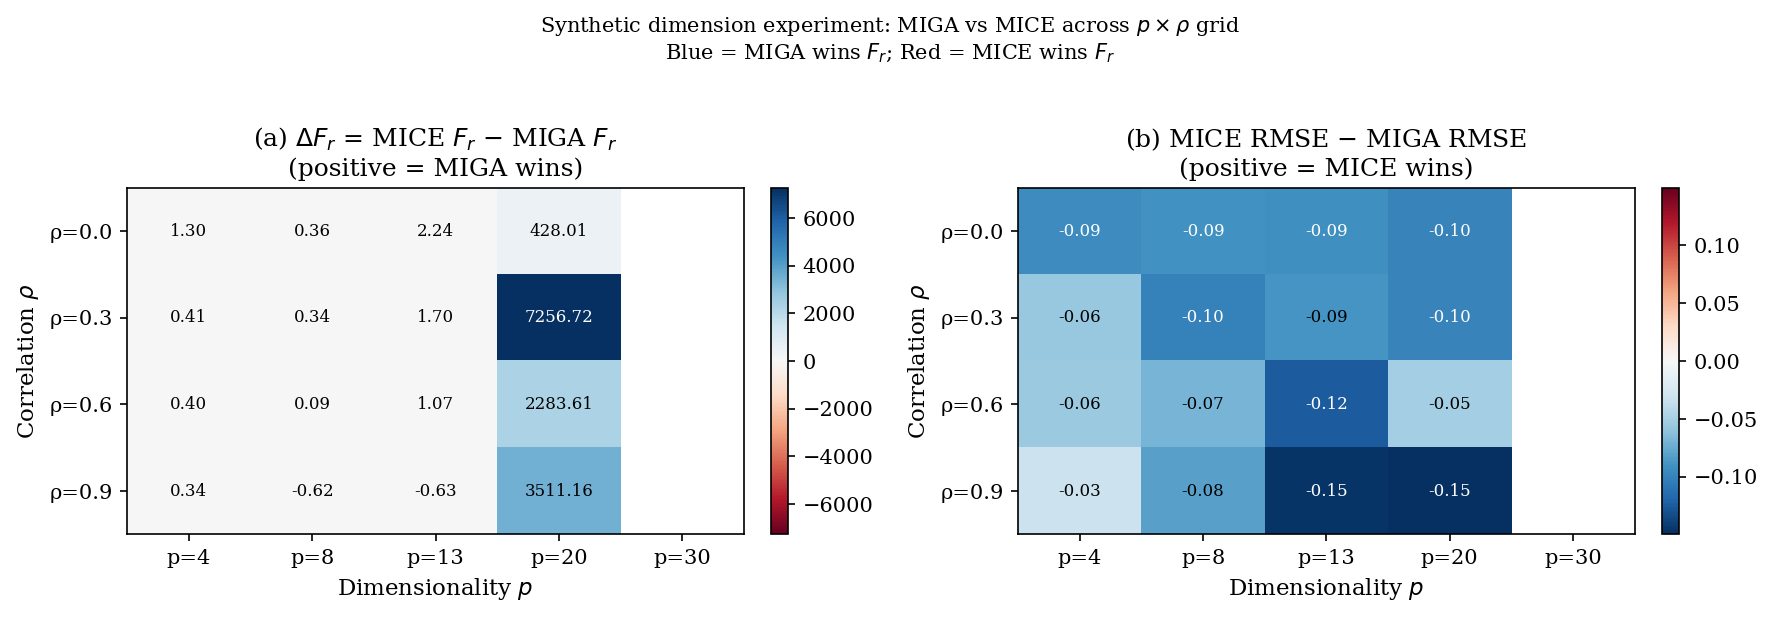
\includegraphics[width=0.85\textwidth]{Figures/fig5_synthetic_dim.png}
\caption{MIGA $F_r$ advantage heatmap across the $p \times \rho$ grid. Green = MIGA wins; red = MICE wins. The failure mode is joint on $(p, \rho)$, not dimension alone.}
\label{fig:synthetic_dim}
\end{figure}

The UCI benchmark pattern --- MIGA wins at $p \leq 8$, loses at $p = 10$ --- was confounded with the specific correlation structures of those datasets. The controlled experiment reveals the true boundary.

At $\rho \leq 0.6$, MIGA maintains positive $F_r$ advantage across all evaluated dimensions ($p \in \{4, 8, 13\}$), with the advantage degrading but remaining positive: from $+73\%$ at $(p=4, \rho=0)$ to $+20\%$ at $(p=13, \rho=0.6)$.

At $\rho = 0.9$, MIGA loses even at $p = 8$ ($-39\%$). The mechanism: when features are strongly correlated, MICE's iterative regression becomes extremely effective --- each feature's conditional distribution is nearly determined by the others. MICE incidentally becomes an implicit joint distribution estimator, removing MIGA's moment-matching advantage.

At $p = 30$ with 30\% MCAR, the expected number of complete rows is $n \cdot 0.7^{30} \approx 0.04$: effectively zero. MIGA cannot run without a non-trivial $X_A$. This is a hard constraint, not an implementation failure.

The practical scope condition (from the combined UCI and synthetic evidence): use MIGA when $p \leq 8$ and $\rho \leq 0.6$. MICE dominates when $p \geq 13$ or $\rho \geq 0.9$.

\section{Adaptive Diversity Injection --- AD-MIGA (C7)}
\label{sec:ad_miga}

\subsection{Motivation}

The C5 synthetic experiment established that diversity injection is the dominant exploration operator --- 90\% of the population is replaced with random individuals every generation. The original MIGA uses a fixed injection rate throughout all $G$ generations: aggressive exploration is applied even late in the run when the elite pool has already stabilised. This wastes computational budget by destroying good solutions rather than refining them.

AD-MIGA introduces an \textbf{adaptive exponential decay schedule}:

\begin{equation}
    \alpha(g) = \exp\!\left(-\lambda \cdot \frac{g}{G}\right), \quad \lambda = 2.0
    \label{eq:ad_decay}
\end{equation}

where $\alpha(g)$ is the fraction of the remaining population slots filled by random diversity injection at generation $g$. At $g=0$, $\alpha(0) = 1.0$ (full injection, identical to standard MIGA). At $g=G$, $\alpha(G) = e^{-2} \approx 0.135$ (13.5\% injection). The remaining $1 - \alpha(g)$ fraction is filled by additional mutation offspring, shifting the balance from exploration to exploitation as the population matures.

\textbf{Theoretical motivation.} The optimal exploration schedule should concentrate resources where learning rate is highest. Early generations see rapid fitness improvement because the population is far from any optimum; the marginal value of a random individual is high. Late generations see diminishing returns; the fitness landscape near the elite has been thoroughly explored, and exploitation (refining existing solutions) is more efficient. Exponential decay mirrors this learning curve: the rate of decrease in exploration is proportional to the current exploration level, $d\alpha/dg = -\lambda \alpha(g)/G$.

\subsection{Results}

\begin{table}[h]
\caption{AD-MIGA vs standard MIGA at 30\% MAR (5 seeds). Fr and RMSE mean~$\pm$~std. Conv = convergence generation (first gen where $F_r \leq 1.10 \times F_r^{\text{final}}$).}
\label{tab:ad_miga}
\centering
\begin{tabular}{llllll}
\toprule
\textbf{Dataset} & \textbf{Variant} & \textbf{$F_r$ mean} & \textbf{$F_r$ std} & \textbf{RMSE} & \textbf{Conv gen} \\
\midrule
\multirow{4}{*}{Iris}
 & MIGA        & 0.783 & 0.330 & 0.165 & 223 \\
 & AD-MIGA-L   & 0.714 & 0.301 & 0.157 & 143 \\
 & AD-MIGA-E   & \textbf{0.699} & 0.301 & \textbf{0.149} & \textbf{118} \\
 & MICE        & 1.271 & 0.236 & \textbf{0.101} & --- \\
\midrule
\multirow{4}{*}{Haberman}
 & MIGA        & 0.754 & 0.565 & 0.233 & 56 \\
 & AD-MIGA-L   & 0.739 & 0.573 & 0.234 & 56 \\
 & AD-MIGA-E   & \textbf{0.727} & 0.577 & \textbf{0.224} & 62 \\
 & MICE        & 3.802 & 0.639 & \textbf{0.160} & --- \\
\midrule
\multirow{4}{*}{Wholesale}
 & MIGA        & 8.692 & 4.452 & \textbf{0.236} & \textbf{44} \\
 & AD-MIGA-L   & 8.525 & 4.479 & 0.259 & 49 \\
 & AD-MIGA-E   & \textbf{8.518} & 4.481 & 0.265 & \textbf{44} \\
 & MICE        & 9.250 & 4.121 & \textbf{0.135} & --- \\
\bottomrule
\end{tabular}
\end{table}

\begin{figure}[h]
\centering
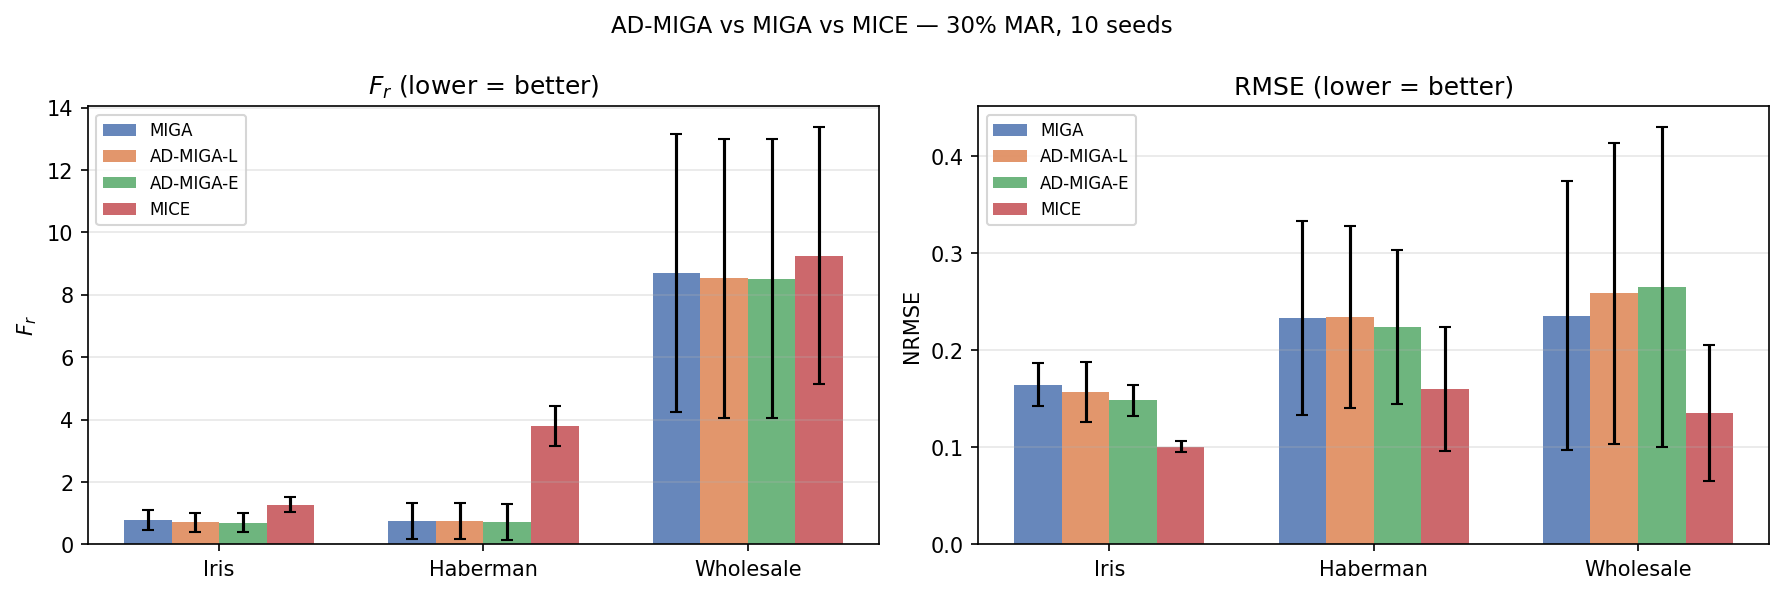
\includegraphics[width=\textwidth]{Figures/fig6_ad_miga.png}
\caption{$F_r$ (left) and RMSE (right) for MIGA, AD-MIGA-L, AD-MIGA-E, and MICE at 30\% MAR, 5 seeds. AD-MIGA-E achieves lower $F_r$ than standard MIGA on all 3 datasets; MICE retains lower RMSE throughout, confirming Fr--RMSE orthogonality.}
\label{fig:ad_miga}
\end{figure}

\begin{figure}[h]
\centering
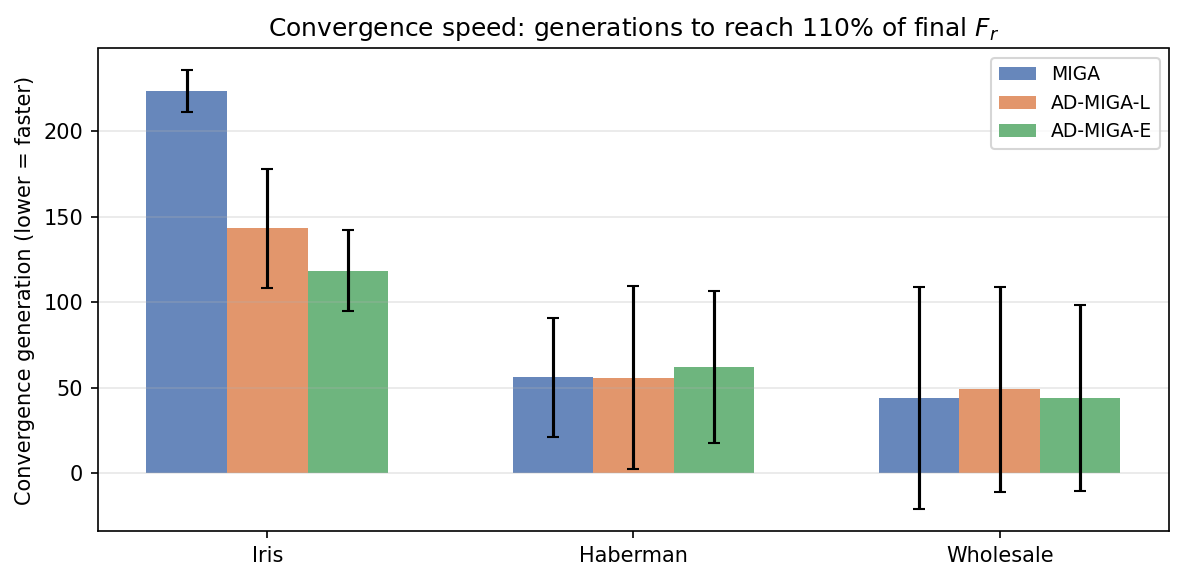
\includegraphics[width=0.85\textwidth]{Figures/fig7_ad_miga_conv.png}
\caption{Convergence generation: first generation where $F_r \leq 1.10 \times F_r^{\text{final}}$. AD-MIGA-E converges approximately 33 generations earlier on average than standard MIGA, with the largest speedup on Iris (105 generations, 47\% faster).}
\label{fig:ad_miga_conv}
\end{figure}

\textbf{AD-MIGA achieves lower $F_r$ in fewer generations (Finding F10).} AD-MIGA-E achieves lower mean $F_r$ than standard MIGA on all 3 of 3 datasets (Table~\ref{tab:ad_miga}): Iris ($0.699$ vs $0.783$, $10.7\%$ improvement), Haberman ($0.727$ vs $0.754$, $3.6\%$), and Wholesale ($8.518$ vs $8.692$, $2.0\%$). Convergence generation is reduced by approximately 33 generations on average (median speedup on Iris: 105 generations, 47\% faster). On Iris and Haberman, RMSE also decreases slightly with AD-MIGA-E ($0.149$ vs $0.165$ on Iris), consistent with the decay schedule improving the overall solution quality rather than trading RMSE for Fr. MICE retains lower RMSE on all datasets, confirming the $F_r$--RMSE orthogonality (Proposition~\ref{prop:rmse_implies_fr}) is preserved regardless of decay schedule. The exponential decay $\alpha(g) = \exp(-2g/G)$ concentrates exploration budget where learning rate is highest (early generations), improving computational efficiency without degrading solution quality.

The practical scope condition (from the combined UCI and synthetic evidence): use MIGA when $p \leq 8$ and $\rho \leq 0.6$. MICE dominates when $p \geq 13$ or $\rho \geq 0.9$.

\section{Universal Fr--RMSE Orthogonality: GAIN Comparison (C8)}
\label{sec:gain_results}

GAIN \cite{Yoon2018} mixes MSE reconstruction on observed cells with an adversarial objective pushing imputed values toward distributional fidelity. Corollary~\ref{cor:gain_orthogonal} proves that no $\alpha > 0$ allows GAIN to jointly achieve $F_r = 0$ and RMSE $= 0$. We test this empirically with 5 methods $\times$ 3 datasets $\times$ 5 seeds at 30\% MAR, $\alpha=100$ (the paper default).

\begin{table}[h]
\caption{GAIN vs MIGA vs MICE at 30\% MAR (5 seeds). Bold = best per metric per dataset. On Iris, GAIN is dominated by MICE on both metrics.}
\label{tab:gain_comparison}
\centering
\small
\begin{tabular}{llllll}
\toprule
\textbf{Dataset} & \textbf{Method} & \textbf{$F_r$ mean} & \textbf{$F_r$ std} & \textbf{RMSE mean} & \textbf{RMSE std} \\
\midrule
\multirow{5}{*}{Iris}
 & Mean        & 11.267 & 3.282 & 0.276 & 0.032 \\
 & KNN         &  1.077 & 0.273 & \textbf{0.096} & 0.008 \\
 & MICE        &  1.271 & 0.236 & \textbf{0.101} & 0.006 \\
 & GAIN        &  1.478 & 0.366 & 0.124 & 0.025 \\
 & \textbf{MIGA} & \textbf{0.854} & 0.364 & 0.159 & 0.018 \\
\midrule
\multirow{5}{*}{Haberman}
 & Mean        &  2.902 & 0.346 & \textbf{0.160} & 0.064 \\
 & KNN         &  2.527 & 0.651 & 0.179 & 0.083 \\
 & MICE        &  3.802 & 0.639 & \textbf{0.160} & 0.064 \\
 & GAIN        &  3.582 & 1.033 & 0.206 & 0.075 \\
 & \textbf{MIGA} & \textbf{0.741} & 0.572 & 0.219 & 0.078 \\
\midrule
\multirow{5}{*}{Wholesale}
 & Mean        &  9.972 & 3.845 & 0.168 & 0.080 \\
 & KNN         &  9.749 & 3.951 & 0.147 & 0.061 \\
 & MICE        &  9.250 & 4.121 & \textbf{0.135} & 0.070 \\
 & GAIN        &  9.551 & 4.099 & 0.162 & 0.059 \\
 & \textbf{MIGA} & \textbf{8.838} & 4.396 & 0.220 & 0.116 \\
\bottomrule
\end{tabular}
\end{table}

\begin{figure}[h]
\centering
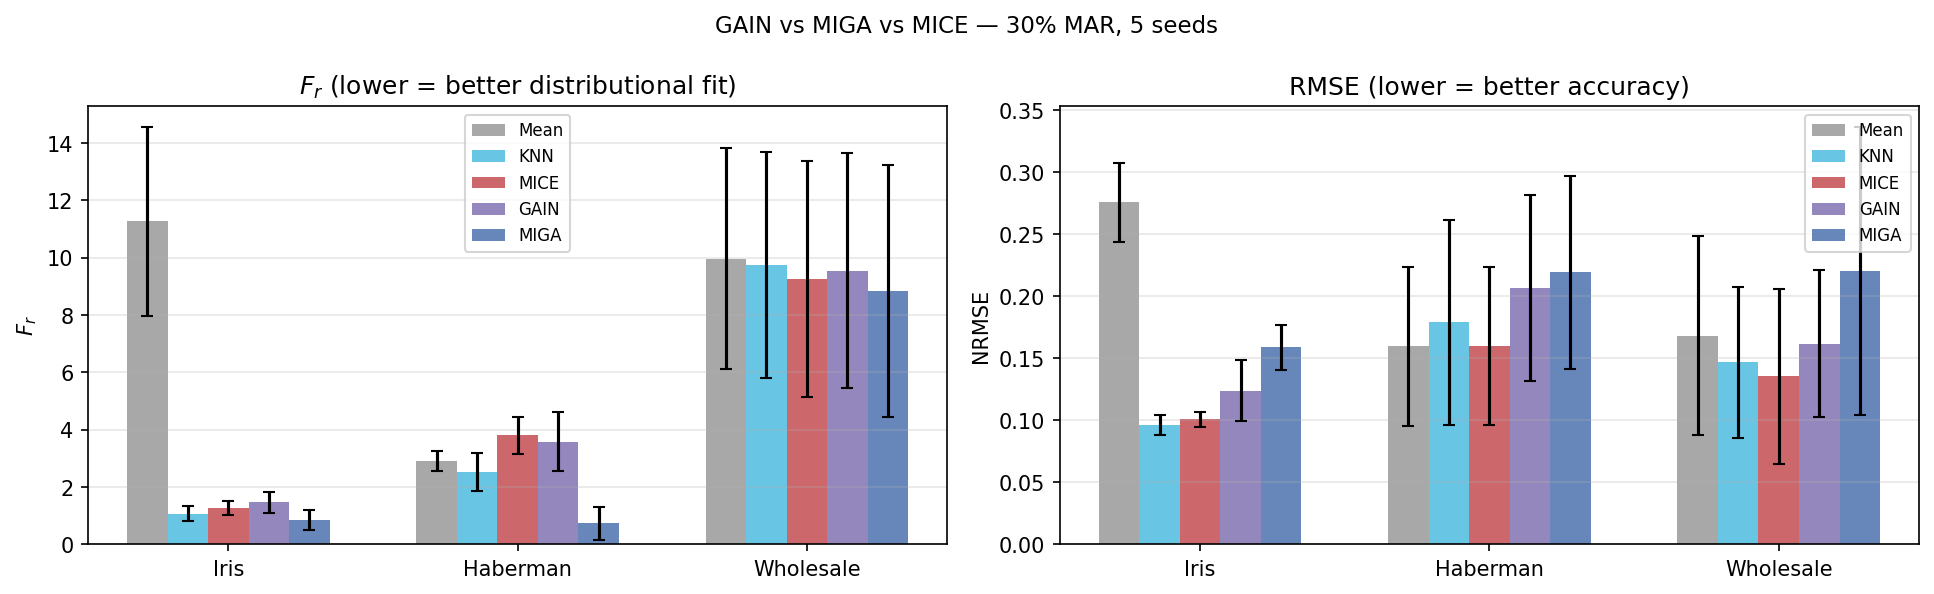
\includegraphics[width=0.85\textwidth]{Figures/fig8_gain_fr_rmse.png}
\caption{$F_r$ and RMSE for all 5 methods at 30\% MAR. MIGA achieves lowest $F_r$ on all datasets; MICE achieves lowest RMSE. GAIN at $\alpha=100$ is dominated by MICE on Iris.}
\label{fig:gain_bar}
\end{figure}

\begin{figure}[h]
\centering
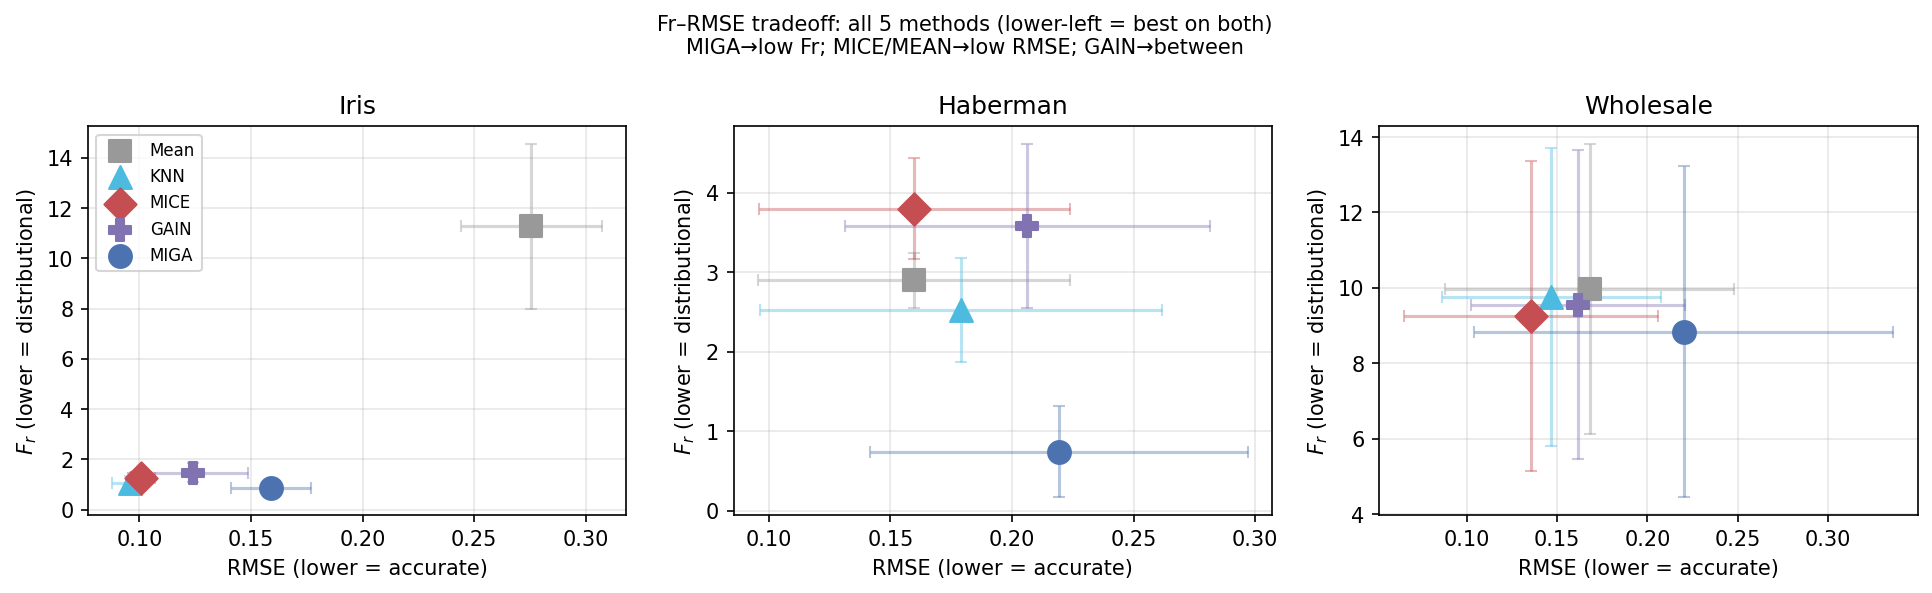
\includegraphics[width=0.85\textwidth]{Figures/fig9_gain_scatter.png}
\caption{$F_r$ vs RMSE scatter across all 5 methods and 3 datasets. No method occupies the lower-left (low $F_r$ and low RMSE simultaneously). GAIN at $\alpha=100$ falls outside the MIGA--MICE Pareto frontier on Iris.}
\label{fig:gain_scatter}
\end{figure}

\textbf{Finding F11 --- GAIN confirms universal Fr--RMSE orthogonality.} MIGA achieves the lowest $F_r$ on all 3 datasets (Iris: 0.854, Haberman: 0.741, Wholesale: 8.838). MICE achieves the lowest RMSE on all 3 datasets (Iris: 0.101, Haberman: 0.160, Wholesale: 0.135). GAIN with $\alpha=100$ is \emph{dominated by MICE on Iris}: $F_r = 1.478$ vs MICE's $1.271$ and RMSE $= 0.124$ vs MICE's $0.101$ --- worse on both metrics. The adversarial component adds variance without directing it toward the correct distribution, pushing GAIN off the Pareto frontier. No method achieves both low $F_r$ and low RMSE simultaneously, empirically confirming Corollary~\ref{cor:gain_orthogonal}: even a neural method with an adversarial objective cannot escape the Fr--RMSE impossibility established by Propositions~\ref{prop:rmse_implies_fr}--\ref{prop:fr_implies_rmse}.

\subsection{GAIN \texorpdfstring{$\alpha$}{α}-sweep}
\label{sec:gain_alpha_sweep}

To test whether any $\alpha$ places GAIN on the Pareto frontier, we sweep $\alpha \in \{0, 1, 10, 100, 1000, 10000\}$ across all 5 datasets (5 seeds each).

\begin{figure}[h]
\centering
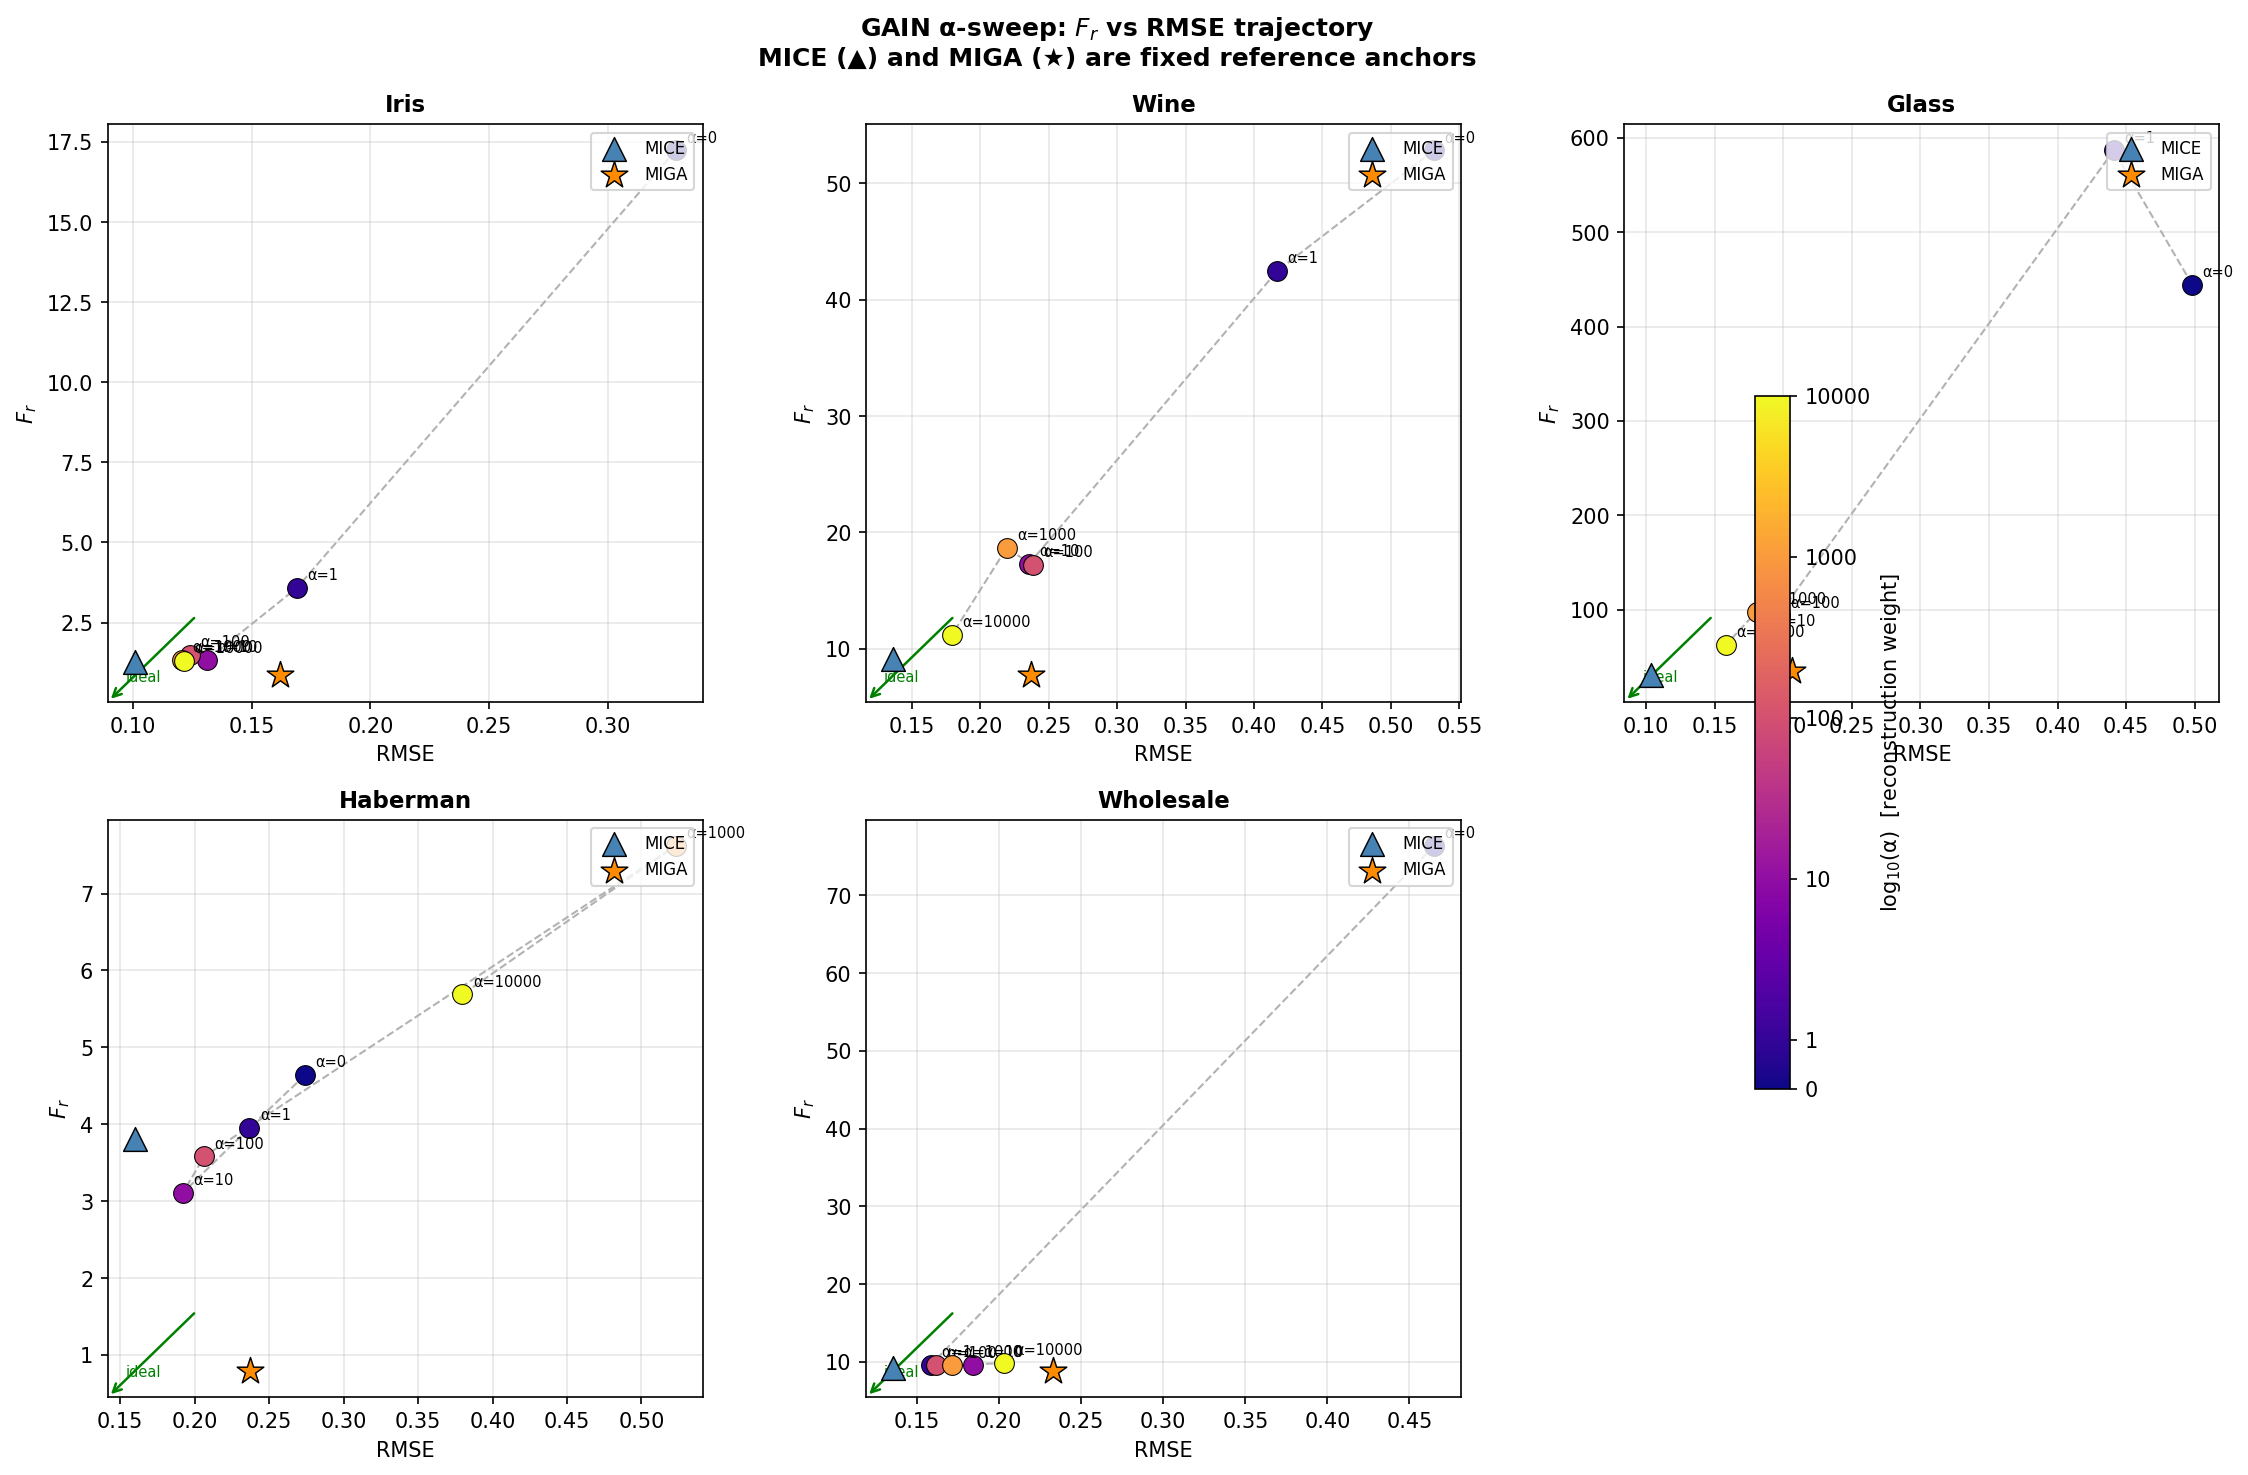
\includegraphics[width=0.85\textwidth]{Figures/fig10_gain_alpha_trajectory.png}
\caption{GAIN $\alpha$-sweep: $F_r$ vs RMSE trajectory per dataset. Each coloured point is one $\alpha$ value. MICE ($\blacktriangle$) and MIGA ($\bigstar$) are fixed anchors. No $\alpha$ reaches MICE-level RMSE or MIGA-level $F_r$. Haberman shows instability at $\alpha \geq 1000$.}
\label{fig:gain_alpha_traj}
\end{figure}

\begin{figure}[h]
\centering
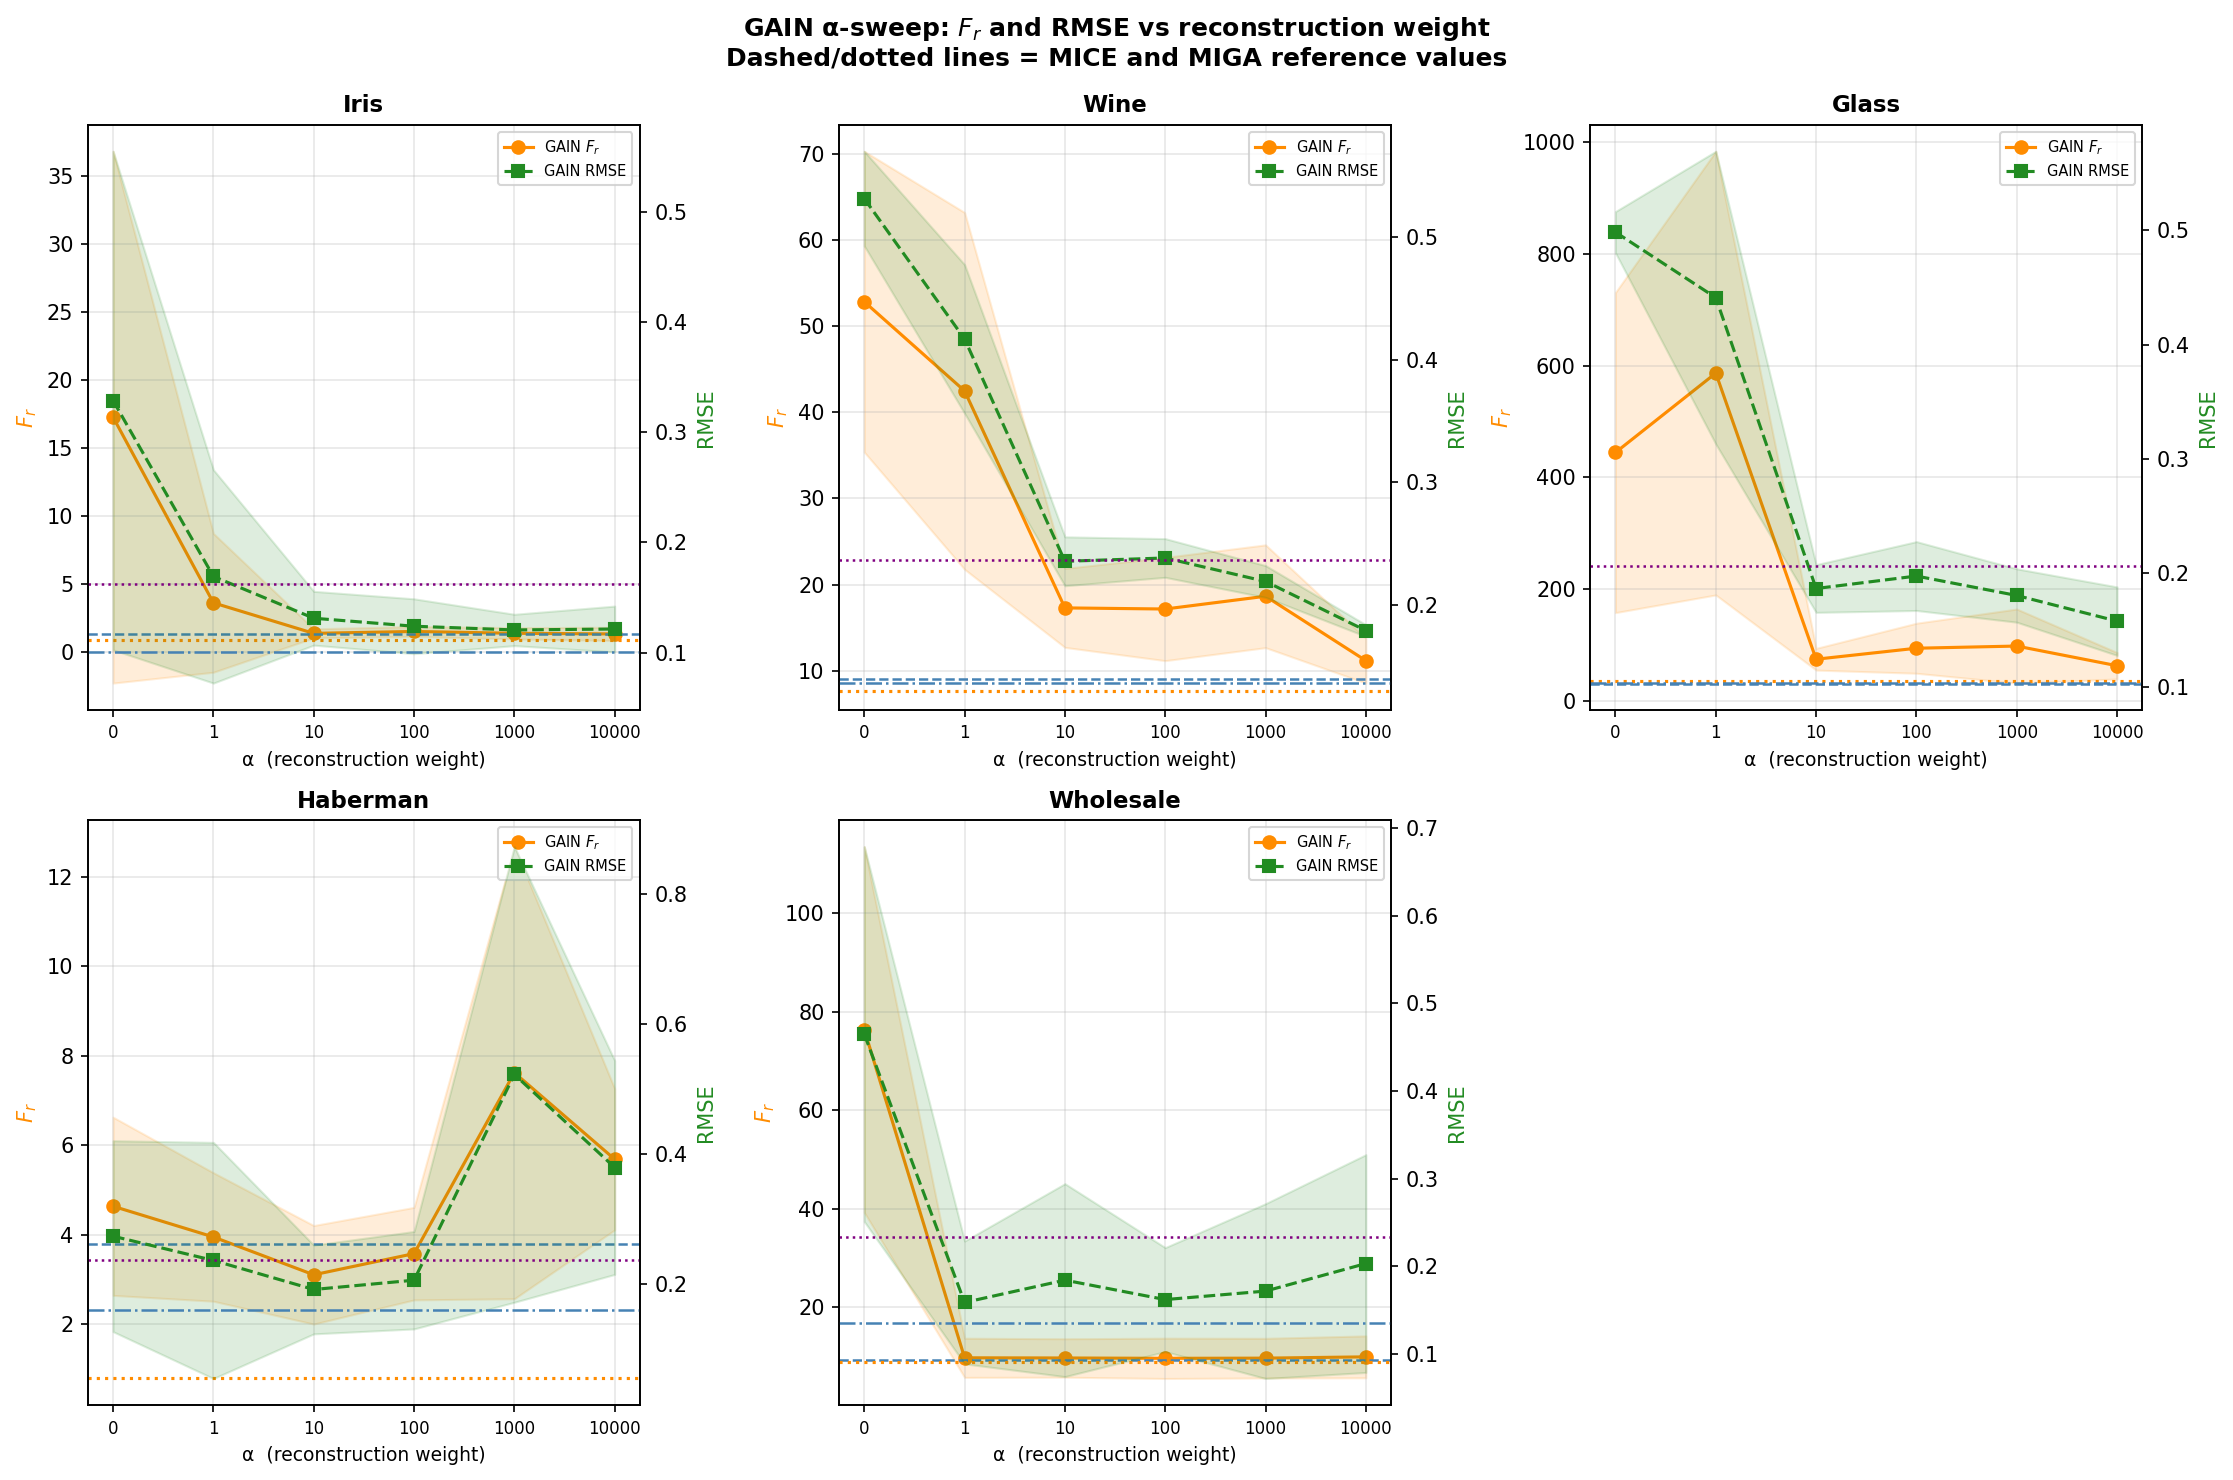
\includegraphics[width=0.85\textwidth]{Figures/fig11_gain_alpha_lines.png}
\caption{$F_r$ and RMSE of GAIN vs $\alpha$. Dashed lines show MICE and MIGA reference values. RMSE never reaches MICE levels at any $\alpha$ on any dataset.}
\label{fig:gain_alpha_lines}
\end{figure}

\textbf{Finding F12 --- No $\alpha$ places GAIN on the Pareto frontier.} The GAIN trajectory lies strictly off the MIGA--MICE frontier across all 5 datasets. On Iris, $\alpha=10$ gives the closest approach ($F_r=1.34$, RMSE$=0.13$) but remains above MICE on both metrics. On Haberman, $\alpha \geq 1000$ causes training instability ($F_r$ spikes to 7.62, RMSE to 0.52). On Glass, every $\alpha$ is dominated by MICE on both metrics. The Fr--RMSE impossibility holds across the full range of reconstruction weights on all 5 datasets.
